%!TEX root = twig.tex

\chapter{The Twig Language}
\label{ch:semantics}

\section{Formal Semantics}
\label{sec:sem:formal}

Twig is based on \emph{System S}~\cite{system-s}, which was
originally designed as a core language for term rewriting
systems~\cite{baader98rewriting}. A review of term rewriting and
System S is given in Section~\ref{sec:background:trs}. In Twig,
use the operators of System S to combine primitive \emph{rules}
into complex expressions. An expression is applied to an input
term, which represents some type in the target language. The
expression may transform the given type, generating code as a side
effect, or the transformation may fail. In this way, different
code can be generated depending on the input term. Twig's
semantics are inspired by Fig~\cite{fig}, but extended to
incorporate our code generation model. In the following sections
we describe this process more formally.

%!TEX root = twig.tex

\subsection{Terms}
\label{sec:terms}

Twig programs operate on values called \emph{terms}. Terms
represent tree-structured data with labeled internal nodes, a
versatile data type useful in a variety of applications. For
example, abstract syntax trees are naturally represented as terms.

We define the grammar for constructing terms as follows:

\[
t \;\mbox{:=}\; x \;|\; c \;|\; f(t_1,\ldots,t_n)
\]

A term is either a variable $x$, a constant $c$, or the
application of a \emph{constructor} $f$ to at least one other
term. In Twig's syntax, constants and constructors can be any
string of characters beginning with a lower-case letter. The only
string excluded from this condition is the special constructor
\texttt{tuple} (see Section~\ref{sec:tuples}, below). Variables
are represented by strings of characters beginning with a capital
letter; in our presentation we will typically use a single capital
letter only, e.g., \texttt{X} or \texttt{Y}. We use a fixed-width
font when presenting terms, e.g., the constant term
\texttt{myterm}, or the constructed term with a variable
\texttt{cons(myterm1,X)}.

Following the notation of System S, we denote the set of all
variables $\mathcal{X}$, and the set of all terms containing
variables $T(\mathcal{X})$. We denote the set of all terms without
variables, known as \emph{ground terms}, as $T$.

In many systems, terms are typed through the use of
\emph{signatures}~\cite{baader98rewriting}. That is, certain terms
can be defined as valid in a particular domain, and terms not
found to conform can be flagged as errors. Twig could be extended
to support term signatures, and indeed this might be useful. In
our current work, however, we consider only untyped terms.

For the purposes of Twig's semantics, the meaning of a particular
term (other than \texttt{tuple}s) is abstract. Terms are defined
by their use in the program's \emph{rules}, described below.


\subsubsection{Tuples}
\label{sec:tuples}

Twig recognizes a special kind of term: tuples. The tuple elements
are represented as the sub-terms of a term with a special
constructor: \texttt{tuple}. Tuples may have any length. Twig's
syntax equates the absence of any constructor with the presence of
the \texttt{tuple} constructor. For example, the syntax
\texttt{(string,int)} is interpreted as the
\texttt{tuple(string,int)}. This term represents a tuple of length
two, whose first element is \texttt{string} and whose second
element is \texttt{int}.

The \emph{size} of a tuple is simply the cardinality of its
children. We will sometimes write $\mathtt{tuple}_n(\ldots)$ to
indicate a tuple of length $n$, where the length is not otherwise
clear from the context.

One complication arises since we permit tuples to be nested to
arbitrary depth. For example the term

\[
\mathtt{tuple(tuple(int,float),tuple(double))} 
\]

is a nested tuple. In our semantics, we will require the
\emph{width} of a tuple, defined as

\[
\mbox{width}(t) = \left\{
  \begin{array}{cl}
    \sum^{i=1}_{n} \mbox{width}(t_i) 
      & \mbox{if } t = \mathtt{tuple}(t_1,\ldots,t_n)\vspace{2mm}\\
    1 & \mbox{otherwise}
  \end{array}
\right.
\]

Intuitively, the width of a tuple corresponds to its size after
being ``flattened,'' where the elements of nested tuples are
pushed up, recursively, to the top level. If we flattened the
tuple in the example above, we would get

\[
\mathtt{tuple(int,float,double)}
\]

and its width would be three.


\subsubsection{Terms representing types}

In Twig, terms are used to represent types in a target language.
For example, we use terms such \texttt{int} and \texttt{float} to
represent primitive types in C. Terms built with constructors can
represent types with some structure, e.g., the term
\texttt{ptr(int)} can represent a C pointer to an integer. More
complicated terms may involve multiple children, and may be nested
to any depth. For example, the term

\[
\mathtt{struct(int,float,struct(ptr(char)))}
\]

can represent a structure with three fields: an \texttt{int}, a
\texttt{float}, and a second structure with a single string
(pointer to \texttt{char}) field.

The mapping between terms and types in the target language is a
configuration option, customizable for a particular domain. The
mapping need not be injective, that is, multiple terms in Twig may
represent a single type in the target language. For example, you
might have the distinct terms \texttt{string} and
\texttt{ptr(char)} both map to a \texttt{char} pointer in C.

%!TEX root = twig-language.tex

\subsection{Expressions}
\label{sec:expressions}

Twig \emph{expressions} can be either \emph{primitive rules}
(Section~\ref{sec:semantics:prims}) or else built from other
expressions using operators (Section~\ref{sec:semantics:ops}). An
expression $s$ maps terms $T$ to elements of the set $(T \times M)
\cup \{\bot\}$, i.e., either a pair $(t',m)$ where $t' \in T$ and
$m$ is a \emph{block} of generated code in the set $M$ (see
Section~\ref{sec:code-gen}), or else the special, distinguished
value $\bot$. Formally, $s$ is a function:

\[
s : T \to ((T \times M) \cup \{\bot\})
\]

Following Fig's notation, we use $\bot$ to denote ``failure.'' In
particular, $\bot$ is used in the semantics for the operators
described in Section~\ref{sec:semantics:ops}.

As with System S and Fig, Twig allows expressions to be named. An
expression's name may be used in place of itself within other
expressions. The syntax is

\[
v \mtt{ = } e
\]

where $v$ is a valid expression name and $e$ is an expression, as
described below. A Twig program is a list of such name/expression
assignments. There is a special expression name, \texttt{main},
which designates the top-level expression for the program.

%!TEX root = twig-language.tex

\subsection{Primitive Rules}
\label{sec:semantics:prims}

The simplest Twig expressions are \emph{primitive rules}, which
describe a single transformation step. Since Twig terms represent
types in a target language, a primitive rule in Twig describes how
to transform an instance of one type into an instance of another
in that language.

The syntax for primitive rules is

\[
\mtt{[} p_1 \mtt{ -> } p_2 \mtt{]} \mtt{<<< } m \mtt{ >>>}
\]

where $p_1$ is the \emph{input pattern}, $p_2$ the \emph{output
pattern}, and $m$ is a block of code (see
Section~\ref{sec:code-gen}). Input and output patterns are terms,
but which can also contain \emph{variables}.

Informally, a primitive rule transforms $t$ to $t'$ with an
associated block $m$ if and only if the application of rule to
value $t$ succeeds. In this case we write $t \arr{s} (t',m)$.
Otherwise, if the application of $s$ to $t$ fails, e.g., if $t$
does not match the input pattern in $s$, then we write $t \arr{s}
\bot$. In this case, the block is not produced.

For example, in C it is easy to convert an integer value to
floating point. Twig's syntax for writing this rule is as follows:

\begin{verbatim}
[int -> float] <<< $out = (float)$in; >>>
\end{verbatim}

In this example, if the input term to the expression
\emph{matches} the term \texttt{int}, then the output of the
expression will be the term \texttt{float} along with a code block
(the text between \texttt{<<<} and \texttt{>>>}, see below). If
the input term does not match \texttt{int} then the output will be
$\bot$.

Input and output patterns can have \emph{variables} in place of
terms or sub-terms. For example the rule

\begin{verbatim}
[ptr(X) -> X] <<< $out = &$in; >>>
\end{verbatim}

describes a transformation of any C pointer type to its referent.
The variable \texttt{X} is bound to the corresponding value of the
matched input on the right, and that value is substituted for the
variable where it appears on the left. Variables may stand in
place of a single term only, not constructors; e.g., patterns such
as \texttt{[X(int)~->~X]} are not allowed.

When an input term is \emph{matched}, we mean that it is
unified~\cite{baader98rewriting} with the input pattern. In fact,
Twig's matching algorithm is simpler than full unification, since
there is no equational theory and the input term may not contain
variables (i.e., must be a ground term). If unification is
successful, we say that the term \emph{matched}. The bound
variables (if any) are saved in order to construct the output term
via substitution. We omit further formalization of matching here
for lack of space; see \cite{baader98rewriting,system-s} for
details.

% Probably should talk about variable binding, e.g. how (X,X) will match a pair of identical terms.

\subsubsection{Blocks}

Primitive rules are associated with have a block. In Twig's syntax, blocks are surrounded by triple-angle braces and appear immediately after a primitive rule, like so:

\begin{verbatim}
[int -> float] <<<
  $out = (float)$in;
>>>
\end{verbatim}

The contents of the block depends on the target language; in this case, we have provided a block of escaped C code (as described in Section~\ref{sec:code-gen:c}). The target language must be specified as a parameter to the Twig runtime (in our current implementation, as a command line option). This means that the text between the \verb|<<<| and \verb|>>>| is interpreted based on the chosen block implementation. A target language specific procedure is passed the text, along with the input and output term(s). It can then construct the block however it sees fit. In our C block implementation, for example, variable names are generated and the terms are used to determine the appropriate types for declaring those variables in a prelude section of the code. Other target languages might choose very different block construction mechanisms.

It is important to understand that Twig's semantics do not require that block contents be checked in any way (although an implementation could do this), and that the code generation procedure is strictly syntactic. This scheme is similar to that used by SWIG~\cite{swig}.

%!TEX root = twig.tex

\subsection{Operators}
\label{sec:semantics:ops}

Expressions can be combined using Twig's operators. In the
following semantics, let $t$ range over terms, $m$ range over
blocks, and $s$ range over expressions, i.e., either a primitive
rule, or else another expression built with operators.

The \emph{sequence} operator, written as an infix semi-colon
(\texttt{;}), chains the application of two rules together by
sending the output of the first to the input of the second. The
combined expression fails if either sub-expression fails. With
this operator, simple rules can be composed into multi-step
transformations. Upon success, the result blocks are combined
sequentially using the block sequence operation (see
Section~\ref{sec:code-gen:seq}). The formal semantics are:

\begin{equation}
\label{S1}
\infer
  {t \arr{s_1;s_2} (t'',m_1+m_2)}
  {t \arr{s_1} (t',m_1) \quad t' \arr{s_2} (t'',m_2)}  
\end{equation}

\begin{equation}
\label{S2}
\infer
  {t \arr{s_1;s_2} \bot}
  {t \arr{s_1} \bot}  
\end{equation}

\begin{equation}
\label{S3}
\infer
  {t \arr{s_1;s_2} \bot}
  {t \arr{s_1} (t',m) \quad t' \arr{s_2} \bot}  
\end{equation}

The sequence operator is associative, that is for any expressions
$f,g,h$, $(f;g);h$ is equivalent to $f;(g;h)$. This allows us to
write expressions like $f;g;h$ without ambiguity. We prove this
fact in Section~\ref{sec:seq-assoc}.

\emph{Left-biased choice}, written as a vertical bar (\texttt{|}),
will attempt to apply the first rule expression to the input, and
if it succeeds then its output is the result. If it fails, it
attempts to apply the second rule instead. This operator allows
different code to be generated depending on the input type.
Formally:

\begin{equation}
\label{C1}
\infer
  {t \arr{s_1|s_2} (t',m_1)}
  {t \arr{s_1} (t',m_1)}
\end{equation}

\begin{equation}
\label{C2}
\infer
  {t \arr{s_1|s_2} (t',m_2)}
  {t \arr{s_1} \bot \quad t \arr{s_2} (t',m_2)}
\end{equation}

\begin{equation}
\label{C3}
\infer
  {t \arr{s_1|s_2} \bot}
  {t \arr{s_1} \bot \quad t \arr{s_2} \bot}
\end{equation}

Like the sequence operators, left-biased choice is associative.
For any expression $f,g,h$, $(f|g)|h$ is equivalent to $f|(g|h)$,
allowing us to write $f|g|h$ without ambiguity. We prove this fact
in Section~\ref{sec:choice-assoc}.

Twig includes a variety of other basic operators. The
\emph{identity} (\texttt{T}) expression will always succeed,
returning its input and an identity block. Conversely,
\emph{failure} (\texttt{F}) will always return \texttt{$\bot$}.

\begin{equation}
\label{SUCC}
\infer
  {t \arr{\mathtt{T}} (t,I)}
  {}  
\end{equation}

\begin{equation}
\label{FAIL}
\infer
  {t \arr{\mathtt{F}} \bot}
  {}  
\end{equation}

The unary operator \emph{test} (\texttt{?}) succeeds only if its
argument succeeds, returning the original term and discarding the
result term and block. This operator is useful for examining a
term's structure without actually making use of its sub-terms.

\begin{equation}
\infer
  {t \arr{?s} (t,I)}
  {t \arr{s} (t',m)}
\end{equation}

\begin{equation}
\infer
  {t \arr{?s} \bot}
  {t \arr{s} \bot}  
\end{equation}

Negation (\texttt{$\lnot$}) also takes a single expression
argument. It succeeds only if its argument fails on the input,
returning the original term.

\begin{equation}
\infer
  {t \arr{\lnot s} \bot}
  {t \arr{s} (t',m)}  
\end{equation}

\begin{equation}
\infer
  {t \arr{\lnot s} (t,I)}
  {t \arr{s} \bot}  
\end{equation}

Twig also provides some operators especially for tuples.

The \emph{congruence} operator applies a tuple of expressions to
the elements of a tuple term, pairwise, and returns a tuple of
results. It fails in case any of the individual rule applications
fail. Upon success, the result block is the parallel composition
(see Section~\ref{sec:code-gen:par}) of the individual result
blocks. The formal semantics are as follows:

\begin{equation}
\label{T1}
\infer
  {\mathtt{tuple}(t_1,\ldots,t_n) \arr{(s_1,\ldots,s_n)} (\mathtt{tuple}(t_1',\ldots,t_n'),m_1 \times \ldots \times m_n)}
  {t_1 \arr{s_1} (t_1',m_1) \quad \cdots \quad t_n \arr{s_n} (t_n',m_n)}
\end{equation}

\begin{equation}
\label{T2}
\infer
  {\mathtt{tuple}(\ldots,t_i,\ldots)\arr{(\ldots,s_i,\ldots)}\bot}
  {t_i \arr{s_i} \bot}
\end{equation}

\begin{equation}
\label{T3}
\infer
  {\mathtt{tuple}(t_1,\ldots,t_m) \arr{(s_1,\ldots,s_n)} \bot 
   \quad\mbox{if}\; m \neq n}
  {}
\end{equation}

\begin{equation}
\label{T4}
\infer
  {t \arr{(s_1,\ldots,s_n)} \bot
  \quad\mbox{if}\; t \neq \mathtt{tuple}(\ldots)}
  {}  
\end{equation}


The family of unary \emph{branch} operators apply a single
expression to one, all, or some of a tuple's elements, depending
on the variant.

The branch operator \texttt{\#one} attempts to apply its parameter
$s$ to a single element: the first element, from left to right,
for which $s$ does not fail. The other elements of the tuple are
unchanged. The expression fails if $s$ fails for each element. The
formal semantics for \texttt{\#one} are as follows:

\begin{equation}
\infer
  {\mathtt{tuple}(\ldots,t_i,\ldots) \arr{\mathtt{\#one}(s)} (\mathtt{tuple}(\ldots,t_i',\ldots),(I \times \ldots \times m_i \times \ldots \times I))}
  {t_i \arr{s} (t_i',m_i)}
\end{equation}

\begin{equation}
\infer
  {\mathtt{tuple}(t_1,\ldots,t_n) \arr{\mathtt{\#one}(s)} \bot}
  {t_1 \arr{s} \bot \quad \cdots \quad t_n \arr{s} \bot}  
\end{equation}

\begin{equation}
\infer
  {t \arr{\mathtt{\#one}(s)} \bot
  \quad\mbox{if}\; t \neq \mathtt{tuple}(\ldots)}
  {}  
\end{equation}


The branch operator \texttt{\#all} applies its parameter $s$ to
each element of a tuple. The expression fails if $s$ fails for any
element. The formal semantics for \texttt{\#all} are:

\begin{equation}
\infer{
  \mathtt{tuple}(\ldots,t_i,\ldots)
  \arr{\mathtt{\#all}(s)}
  (\mathtt{tuple}(\ldots,t_i',\ldots),
  (m_1 \times \ldots \times m_n))
}{
  t_1 \arr{s} (t_1',m_1) \quad \cdots \quad t_n \arr{s} (t_n',m_n)
}
\end{equation}

\begin{equation}
\infer
  {\mathtt{tuple}(\ldots,t_i,\ldots) \arr{\mathtt{\#all}(s)} \bot}
  {t_i \arr{s} \bot}  
\end{equation}

\begin{equation}
\infer
  {t \arr{\mathtt{\#all}(s)} \bot
  \quad\mbox{if}\; t \neq \mathtt{tuple}(\ldots)}
  {}  
\end{equation}


The branch operator \texttt{\#some} applies its parameter $s$ to
at least one element of a tuple. The expression fails if $s$ fails
for each elements. The formal semantics for \texttt{\#some} are:

\begin{equation}
\infer{
  \mathtt{tuple}(t_1,\ldots,t_n)
  \arr{\mathtt{\#some}(s)}
  (\mathtt{tuple}(P(t_1),\ldots,P(t_n)),
   Q(t_1) \times \ldots \times Q(t_n))
}{
\begin{array}{l}
P(t) = \left\{
  \begin{array}{l l}
    t' & \quad \text{if}\; t \arr{s} (t',m) \\
    t  & \quad \text{if}\; t \arr{s} \bot \\
  \end{array}\right.\\
Q(t) = \left\{ 
  \begin{array}{l l}
    m & \quad \text{if}\; t \arr{s} (t',m) \\
    I & \quad \text{if}\; t \arr{s} \bot \\
  \end{array}\right.\\
\exists{i} : i \in \{1..n\} \;\wedge\; t_i \arr{s} (t'_i,m)\\
\end{array}
}
\end{equation}

\begin{equation}
\infer
  {\mathtt{tuple}(t_1,\ldots,t_n) \arr{\mathtt{\#some}(s)} \bot}
  {t_1 \arr{s} \bot \quad \cdots \quad t_n \arr{s} \bot}
\end{equation}

\begin{equation}
\infer
  {t \arr{\mathtt{\#some}(s)} \bot
  \quad\mbox{if}\; t \neq \mathtt{tuple}(\ldots)}
  {}  
\end{equation}


A \emph{projection} extracts a single indexed element from a
tuple, discarding the other tuple elements. The formal semantics
are:

\begin{equation}
\infer
  {\mathtt{tuple}(\ldots,t_i,\ldots) \arr{\#i} (t_i,\Pi(i))}
  {}  
\end{equation}

\begin{equation}
\infer
  {\mathtt{tuple}(t_1,\ldots,t_n) \arr{\#i} \bot
  \quad\mbox{if}\; i > n}
  {}  
\end{equation}

\begin{equation}
\infer
  {t \arr{\#i} \bot
  \quad\mbox{if}\; t \neq \mathtt{tuple}(\ldots)}
  {}  
\end{equation}

The \emph{path} unary operator applies a rule to a single
indexed tuple element, leaving the other elements unchanged.

\begin{equation}
\infer
  {\mathtt{tuple}(\ldots,t_i,\ldots) \arr{\#i(s)} (\mathtt{tuple}(\ldots,t_i',\ldots), I \times \ldots \times m_i \times \ldots \times I)}
  {t_i \arr{s} (t_i',m_i)}
\end{equation}

\begin{equation}
\infer
  {\mathtt{tuple}(\ldots,t_i,\ldots) \arr{\#i(s)} \bot}
  {t_i \arr{s} \bot}
\end{equation}

\begin{equation}
\infer
  {\mathtt{tuple}(t_1,\ldots,t_n) \arr{\#i(s)} \bot
  \quad\mbox{if}\; i > n}
  {}  
\end{equation}

\begin{equation}
\infer
  {t \arr{\#i(s)} \bot
  \quad\mbox{if}\; t \neq \mathtt{tuple}(\ldots)}
  {}  
\end{equation}

The \emph{permutation} operator allows arbitrary permutation of a
tuple's elements, including duplicating or dropping elements. The
operator is parameterized by the width of the input tuple and a
list of indices into the tuple. The output will rearrange the
elements of the tuple in the order of the indices. The expression
will fail if the input does not have the given width, or if the
input is not a tuple.

\begin{equation}
\begin{array}{c}
\infer
  {\mathtt{tuple}(t_1,\ldots,t_n) \arr{\mathtt{\#permute}_n(x_1,\ldots,x_m)} (\mathtt{tuple}(t_{x_1},\ldots,t_{x_m}),\Pi_w(y_{x_1},\ldots,y_{x_m}))}{}\\
\mbox{where}\\
\begin{array}{rll}
    & & \{x_1..x_m\} \in \mathbb{N}\\
w   &=& \sum_{j=1}^n \mbox{width}(t_i)\\
b_i &=& \left\{
  \begin{array}{cl}
    0 & \mbox{if } i = 1\\
    \sum_{j=1}^{i-1} \mbox{width}(t_i) & \mbox{if } i > 1
  \end{array}
\right.\\
y_i &=& b_i+1,\ldots,b_i + \mbox{width}(t_i)
\end{array}
\end{array}
\end{equation}

\begin{equation}
\infer
  {\mathtt{tuple}(t_1,\ldots,t_m) \arr{\#\mathtt{permute}_n(\ldots)} \bot
  \quad\mbox{if}\; m \neq n}
  {}  
\end{equation}

\begin{equation}
\infer
  {t \arr{\#\mathtt{permute}_n(\ldots)} \bot
  \quad\mbox{if}\; t \neq \mathtt{tuple}(\ldots)}
  {}  
\end{equation}

The \texttt{\#permute} operator has relatively complex rules for constructing
the result block. This is because blocks must account for each element of a
tuple with a separate input and output. The \texttt{\#permute} operator, by
contrast, rearranges the top-level tuple but must preserve the ordering of
elements within sub-tuples. Figure~\ref{fig:permute} shows the application of
$\mathtt{\#permute}_4(4,3,2,1)$ to the tuple term $((t1,t2,t3),t4,(t5,t6),t7)$
-- the top-level tuple elements are permuted, while in the interior tuples,
ordering is preserved.

\begin{figure}[ht]
\centering
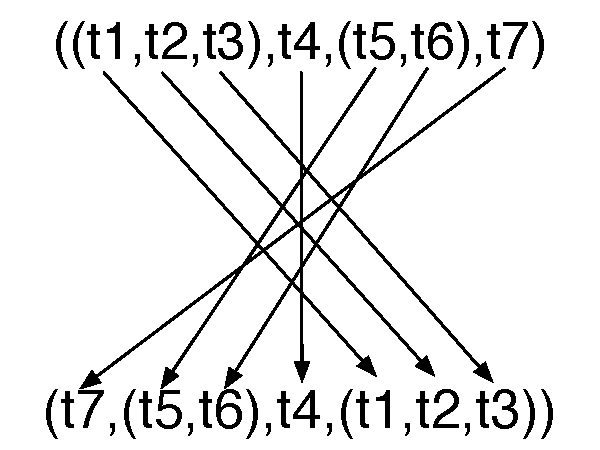
\includegraphics[width=2in]{images/permute}
\caption{Permutation of tuples.}
\label{fig:permute}
\end{figure}

The \texttt{\#fan} operator takes a integer parameter $n$, and
replicates the input term $n$ times in an $n$-element tuple. It is
similar to \texttt{\#permute} but does not require that its input
be a tuple.

\begin{equation}
\begin{array}{c}
\infer
  {t \arr{\mathtt{\#fan}(n)} (\mathtt{tuple}(t,\overset{n}{\ldots},t),\Pi_w(y,\overset{n}{\ldots},y))}
  {}\\
\mbox{where}\\
w = \mbox{width}(t)\\
y = 1,\ldots,w
\end{array}
\end{equation}

The fixed-point operator, \texttt{\#fix}, allows Twig to express
rules for handling recursively defined data types like lists and
trees. An application of $x$ within the expression
$\mathtt{\#fix}_x(s)$, that is, $x$ appearing within $s$, is
essentially a recursive call to the expression
$\mathtt{\#fix}_x(s)$.

\begin{equation}
\infer
  {t \arr{\mathtt{\#fix}_x(s)} (t',m)}
  {t \arr{s[x \mapsto \mathtt{\#fix}_x(s)]} (t',m)}
\end{equation}

\begin{equation}
\infer
  {t \arr{\mathtt{\#fix}_x(s)} \bot}
  {t \arr{s[x \mapsto \mathtt{\#fix}_x(s)]} \bot}
\end{equation}

